\documentclass[11pt, oneside]{article}
\usepackage{latexrc}
\usepackage{hyperref}
\usepackage{float}

\title{CS3110 Hnefatafl Design Doc}
\author{Elizabeth VanDenburgh (eav38)\and Joseph Dwyer (jmd456)\and Taeer Bar-Yam (tb442)}
\date{November, 12 2015}

\begin{document}

\maketitle

\section{Hnefatafl Game Dynamics}
The game is played on an $11\times 11$ checkered board with two uneven sides.
$12$ white pieces are positioned around a white ``king'' at the center of the
board, with $24$ black pieces arranged on the edges surrounding them.
See~\ref{fig:initial_position}.
\begin{figure}\label{fig:initial_position}
  \centering
  \scalebox{.5}{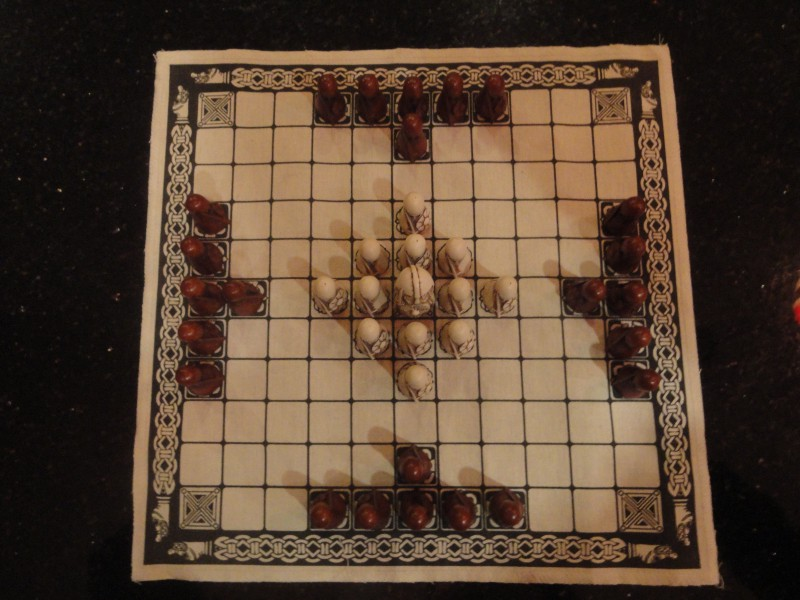
\includegraphics{hnefatafl}}
  \caption{Hnefatafl starting board position. Source: \url{https://medium.com/war-is-boring/you-have-to-play-this-1-600-year-old-viking-war-game-cef088ae4e2d\#.10kof827g}}
\end{figure}
There are three main mechanics involved in the game:
\begin{enumerate}
\item \textbf{Movement}\\
  Pieces move like rooks in chess (horizontally or vertically).
  Only the king has a limited motion of three squares at a time.
\item \textbf{Capturing}\\
  When a piece is flanked by two pieces of the opposing color, that piece is
  ``captured'' and is removed from the board.  This flanking must be done
  actively by the offense (i.e. the center piece can move between the others
  without being captured).\\
  The king cannot participate in flanking an opponent. In the case of the king,
  it must be flanked on all sides to be considered ``captured.''
\item \textbf{Winning}\\
  Black wins when the king is captured, or the king's only escape is to move
  back to the center square of the board.\\
  White wins when the king is moved to one of the side squares of the board.
\end{enumerate}
See: \url{https://en.wikipedia.org/wiki/Tafl\_games\#Hnefatafl}
\section{Interface:}
Ultimately we would like to implement the interface as a GUI using openGL, and
allow click-and-drag motion commands. Initially, we will implement a text-based
interface that uses chess-like notation for movement and output a ASCII grid to
show positions of pieces. This interface will likely remain available as an
option\\
This will be playable against another human player, or against an AI.

\section{Architecture}
\begin{figure}[H]\label{fig:CCD}
  \centering
  \scalebox{0.5}{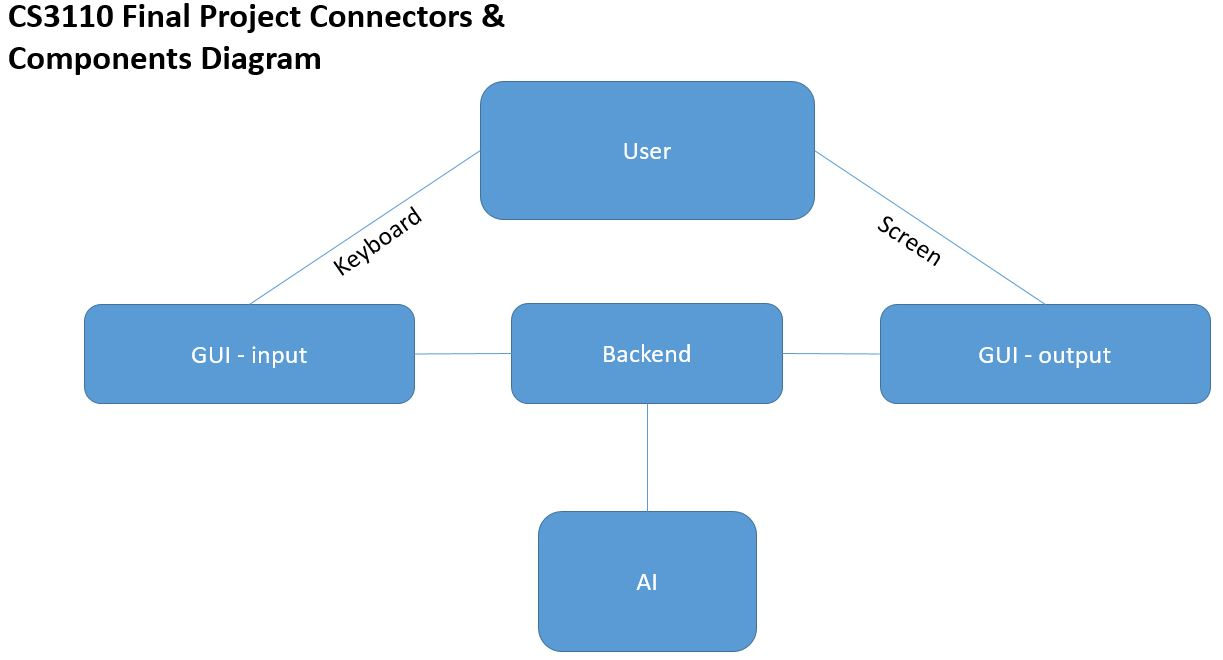
\includegraphics{CCD}}
  \caption{Connector Component Diagram of the pipe and filter architecture for
    our project. Unmarked lines represent connections via function calls
    (APIs).}
\end{figure}
The backend forms a pipe-and-filter architecture that applies an attempted move
to the board state given the rules of the game. The backend and AI components
form a server-client like connection where the backend communicates with the AI
code to determine what the best move is. In this case the AI is the server and
the backend is the client. See~\ref{fig:CCD} for the connector and component
diagram.

\section{System Design}
\begin{figure}[H]\label{fig:MDD}
  \centering
  \scalebox{0.5}{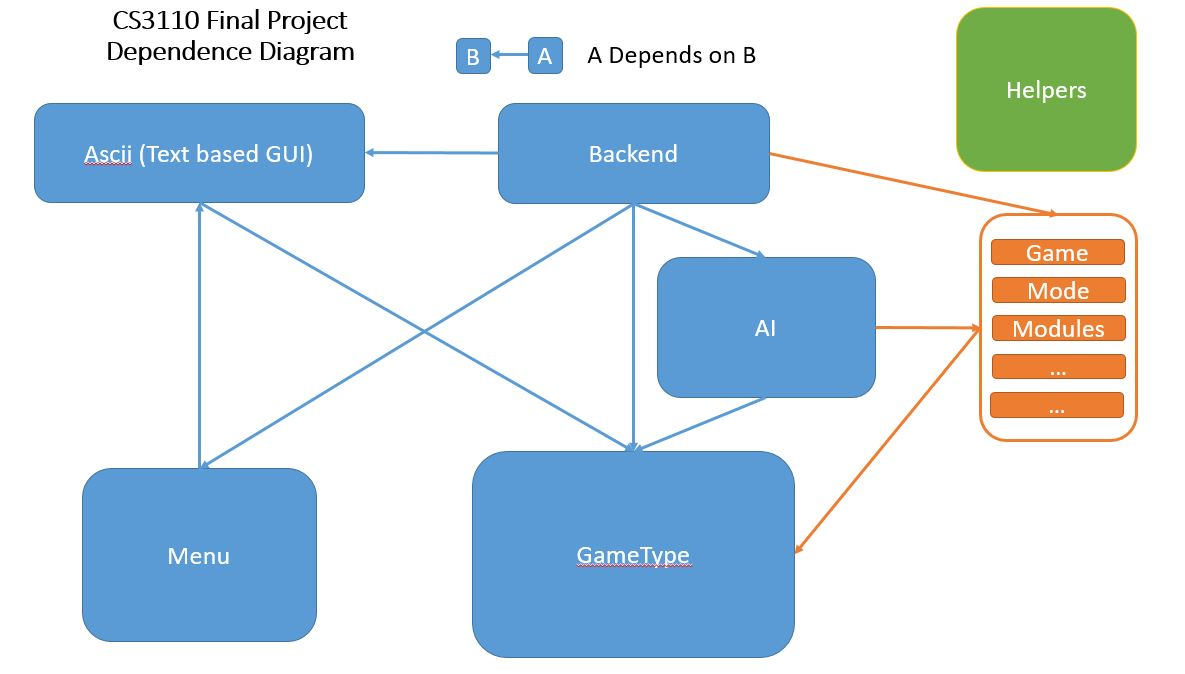
\includegraphics{MDD}}
  \caption{Diagram of dependencies between modules in our project. The helpers
    module (green) is depended on by everything. The game mode modules (orange)
    may or may not end up in the final version}
\end{figure}

\subsection{GUI}
Two options of GUI modules: Text-based and graphical.\\
The purpose of this module is to enable interaction between the user and the
backend. The GUI does none of the game or board computations. It only has
knowledge of the screen state, and what the backend tells it to print. It
\textbf{is} in charge of interpreting piece movement by the user. That is, it
does not report every keystroke, mouseclick, etc. the user makes, only what move
the user would like to make.

\subsection{Backend}
Backend is in charge of the following tasks:
\begin{itemize}
\item Initialization of menu and storage of configuration options
\item Keeps track of the baord and player state
\item Validates moves from the GUI
\item Calculates if a move resulted in a piece's capture
\item Calculates if the game is over and who won
\item Calculates if the game is unwinable (hopefully)
\item Prompts the GUI for the user's next move
\item Prompts the AI for it's next move
\end{itemize}

\subsection{Menu}
In the Menu module is what text to display in the start of game menus. It tells
the GUI which menus to display and the GUI responds with which selection the
user made. The menu composes a game configuration based on the choices and
passes that back to the Backend.\\
Menu will also present a ``Do you want to quit?'' type message on quit.

\subsection{AI}
If playing as one person, the AI module will be passed the current board state
by the Backend. Using this, it will create a decision tree and decide on an
``intelligent'' move
to execute.\\
We can put the AI calls in a separate thread to allow more computation for a
smarter AI.\\\\
Ideally we would like to create either a general AI for all game modes or a
stronger AI for each individual game mode. Based on the amount of time that we
have, and the complexity of building such AI, we will decide which AI
implementation to use.

\subsection{Helpers}
Basic functions that either we feel should have been included in OCaml or most
modules will need are included in Helpers.

\subsection{GameType}
GameType includes basic types for the board, pieces on the board, and other
game-state related objects. It also includes small helper functions that relate
to those types. (e.g. piece\_at for the piece at a location on the board)

\subsection{GameModes?}
We have two ideas for how to implement variants on the game mode (e.g.
differences in win conditions, valid movements, etc.). One involves dynamically
loading one of a set of module that will contain functions for these aspects of
the game.\\
The alternative would be to load preferences out of a plain text file.\\\\
\textit{Pros/Cons:}
\begin{description}
\item[+] Doesn't require us to write text parsing code
\item[+] More flexible (can run arbitrary code)
\item[-] Less secure (can run arbitrary code)
\item[-] Dynamically loading modules is awkward
\end{description}

\section{Module Design}
See attached .mli files.

\section{Data}
Structures include:
\begin{itemize}
\item Piece types (variant)
\item Coordinates (type synonym for int * int)
\item Action variant (what actions the user can perform)
\item Game configurations
\item Board with dimensions and list of piece locations
\end{itemize}

State data:
\begin{itemize}
\item Which player's turn it is
\item Current board state
\item Which game configuration was selected
\end{itemize}
The GUI also stores the current selected piece (the piece the user would like to
move) until the user selects a location to move it to.

Everything is passed through function calls. There is no imperative or global
data.

\section{External Libraries}
\begin{itemize}
\item Termbox for creating an ascii board
\item OpenGL for creating a more graphical gui
\item Potentially Dynlink for dynamically linking game modes
\end{itemize}

\section{Testing Plan}
\begin{itemize}
\item Write unit tests for state of the board after certain moves
  \begin{itemize}
  \item Valid moves
  \item Invalid moves
  \item Win conditions
  \item Piece removal conditions
  \item All of these, in various game modes
  \end{itemize}
\item Watch the AI play against itself
\item Get play testers
\end{itemize}

\section{Stretch Goals:}
\begin{itemize}
\item Hnefatafl is an old game, and there are many versions of it that exist.
  Time permitting, we would like to implement many of these variants, working
  off of a general game core.
\item Detect if the game has become unwinnable.
\item Collecting statistics on the game (who won, how many turns it took, etc)
\item Storing the state of the game at every turn, and enabling turn by turn
  playback
\end{itemize}

\end{document}
